\section{Specifications for the LUC-OS}
\label{sec:lucos}

\begin{figure*}
	\centering
	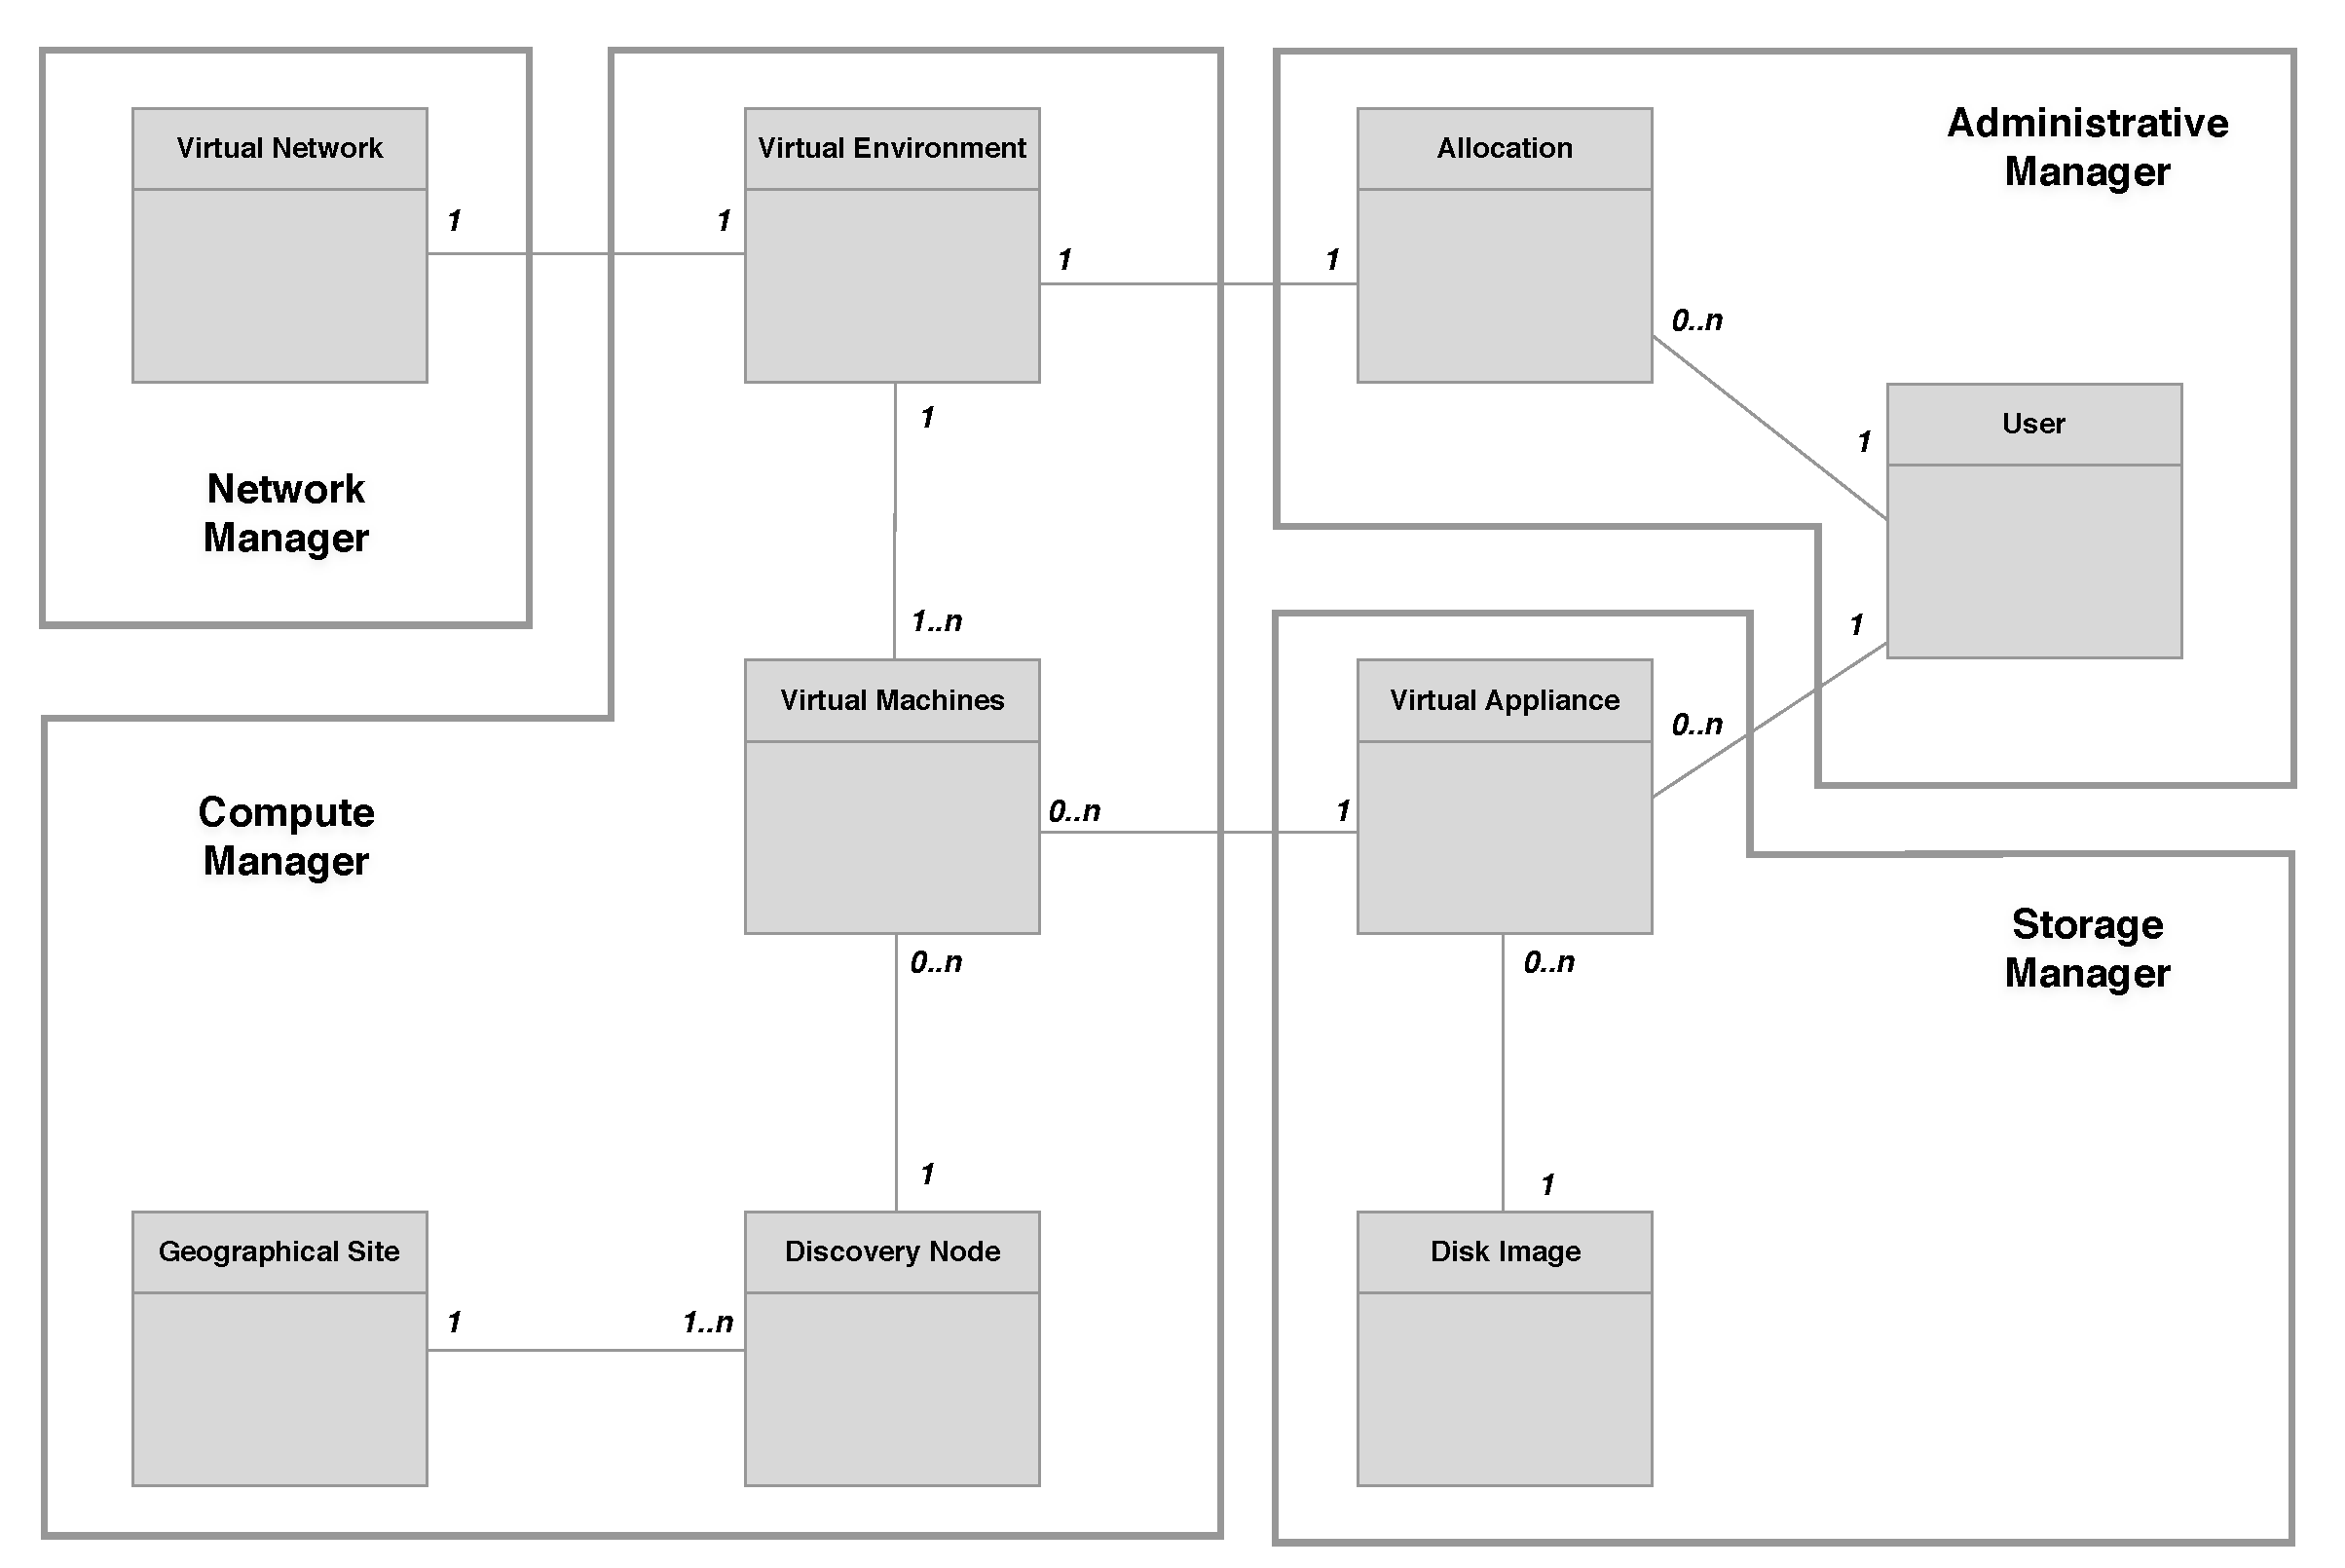
\includegraphics[width=0.91\linewidth]{Figures/mcd_3.pdf}
	\caption{Conceptual schema of entities manipulated by the LUC-OS.}%
	\label{fig:mcd}%
	%\vspace*{-.8cm}
\end{figure*}

In section \ref{sec:moreno} challenges for building massively distributed clouds
over geographically spread infrastructure have been introduced. However 
designing a Cloud OS working over a geographically distributed infrastructure is
quite different from targeting a concentrated context as in data-centers: in
a highly distributed context collaboration between constituting nodes of the 
system deeply depends of network parameters such as latency or bandwidth. 

We deeply think that a system aware of such parameters likely will have a better
reactivity by taking efficient decisions. Locality properties may be introduced
by promoting collaboration between servers that have low latency or high 
bandwidth.

For this reason, we propose to design a locality based utility computing (LUC)
operating system (LUC-OS) for operating massively distributed clouds. To work at
this large scale, it will leverage a locality aware overlay network (LBO), thus 
improving reactivity of service by taking into account networking parameters. 
Leveraging the model introduced in section \ref{sec:moreno} by 
\cite{moreno2012iaas}, we propose a first draft of the LUC-OS architecture: each
of its fundamental services is described in the following listing:

\label{sub:sec:list_services}

\begin{description}

	\item [Compute service] : manages virtual machines' life-cycle.

	\item [Network service] : manages virtual networks over multi-sites.

	\item [Storage service] : manages images and virtual machines' snapshots.

	\item [Administrative service] : manages infrastructure and users' permissions.  

\end{description}

In figure \ref{fig:mcd} we propose a conceptual schema that enables an easier 
illustration of data entities with their relationships, that we plan to use in
the LUC-OS. This is a high-level description which aims at defining and 
explaining semantics of our proposal. It is noticeable that this schema is 
partitioned in four block corresponding to the four services previously exposed.

As entities that will be manipulated by services of the LUC-OS are known, an
overview of how entities are involved during virtual machines provisioning can
be given:

\begin{itemize}

	\item A user asks the LUC-OS to provision some computing resources at a 
	specified date:  the \textbf{administrative service} considers the demand 
	and determine  whether it is possible to provide requested resources or not. 
	Once the demand is considered as acceptable, an allocation is created and 
	stored in the  LUC-OS's data structure (a Distributed Hash Table). To enable
	accounting operations such as billing, the allocation will be stored long
	enough.

	\item Once the allocation date has been reached, the \textbf{compute
	service} will ask the resource scheduler (DVMS) to elect a 
	set of servers that is suitable to spawn the virtual machines, leading to 
	the creation of a new virtual environment which is distributed on the 
	elected servers. \textbf{Network service} then create a new virtual	network
	that is attached to the virtual	environment: during their creations, virtual
	machines will be inter-connected through this virtual network.

	\item The \textbf{storage service} is involved in processes for creating and 
	snapshotting virtual machines. As virtual machine are created from a virtual
	disk image, users will have to specify a virtual appliance (a disk image 
	base flavored with some pre-installed software). Once a virtual machine is 
	started, it is possible for users to snapshot it: the virtual machine state
	is saved in the distributed data structure.

\end{itemize}